% This file was created by matlab2tikz.
%
\definecolor{mycolor1}{rgb}{0.00000,0.44700,0.74100}%
%
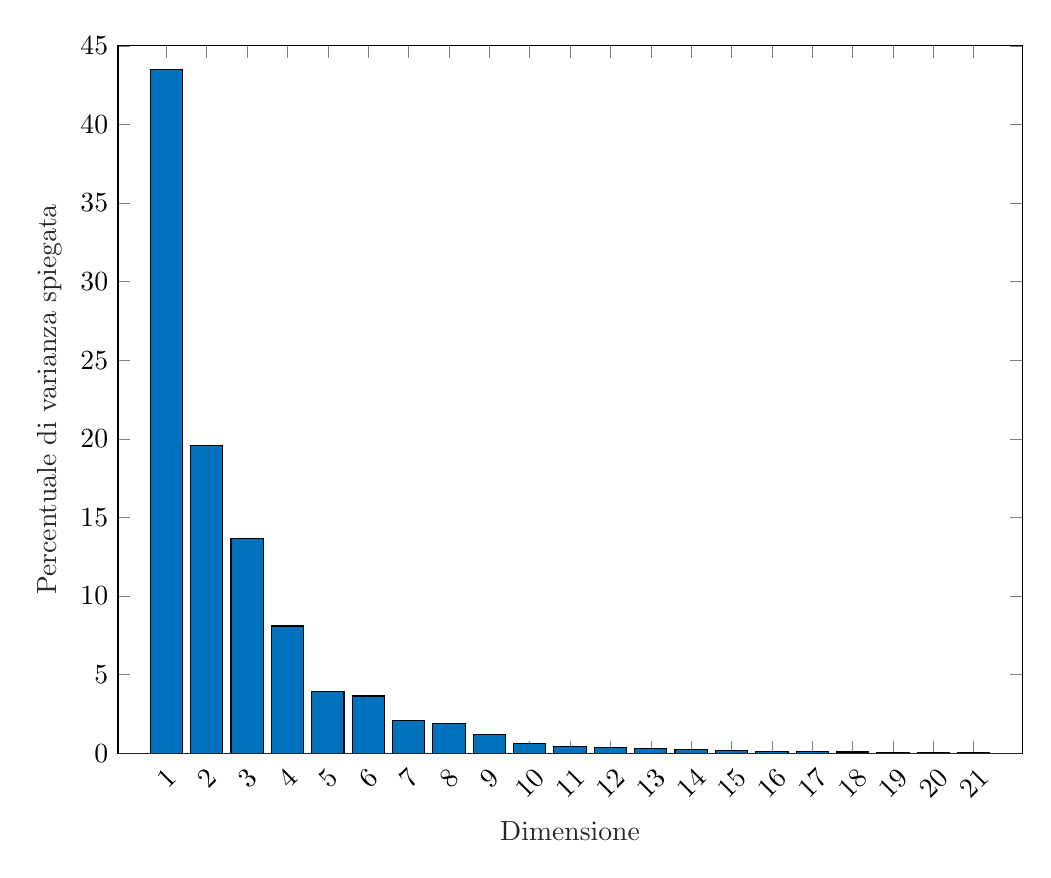
\begin{tikzpicture}

\begin{axis}[%
width=4.521in,
height=3.537in,
at={(0.758in,0.509in)},
scale only axis,
bar shift auto,
xmin=-0.2,
xmax=22.2,
xtick={ 1,  2,  3,  4,  5,  6,  7,  8,  9, 10, 11, 12, 13, 14, 15, 16, 17, 18, 19, 20, 21},
xticklabel style={rotate=45},
xlabel style={font=\color{white!15!black}},
xlabel={Dimensione},
ymin=0,
ymax=45,
ylabel style={font=\color{white!15!black}},
ylabel={Percentuale di varianza spiegata},
axis background/.style={fill=white}
]
\addplot[ybar, bar width=0.8, fill=mycolor1, draw=black, area legend] table[row sep=crcr] {%
1	43.5188772941956\\
2	19.5468901188242\\
3	13.6729006251231\\
4	8.09379237076398\\
5	3.92033031074876\\
6	3.63676576245848\\
7	2.06352857806647\\
8	1.88618546001113\\
9	1.17889356655643\\
10	0.624733591992837\\
11	0.399100475607163\\
12	0.341095270869467\\
13	0.313970334751129\\
14	0.20960802082708\\
15	0.148808269235073\\
16	0.1226872495579\\
17	0.0898938525110919\\
18	0.0747075276186473\\
19	0.0562740676717445\\
20	0.0330050036723956\\
21	0.0206044928991938\\
};
\addplot[forget plot, color=white!15!black] table[row sep=crcr] {%
-0.2	0\\
22.2	0\\
};
\end{axis}
\end{tikzpicture}%